%%% Local Variables:
%%% mode: latex
%%% TeX-master: "../main"
%%% End:

\part{Results and Experiments}

\begin{figure}[H]
  \centering
  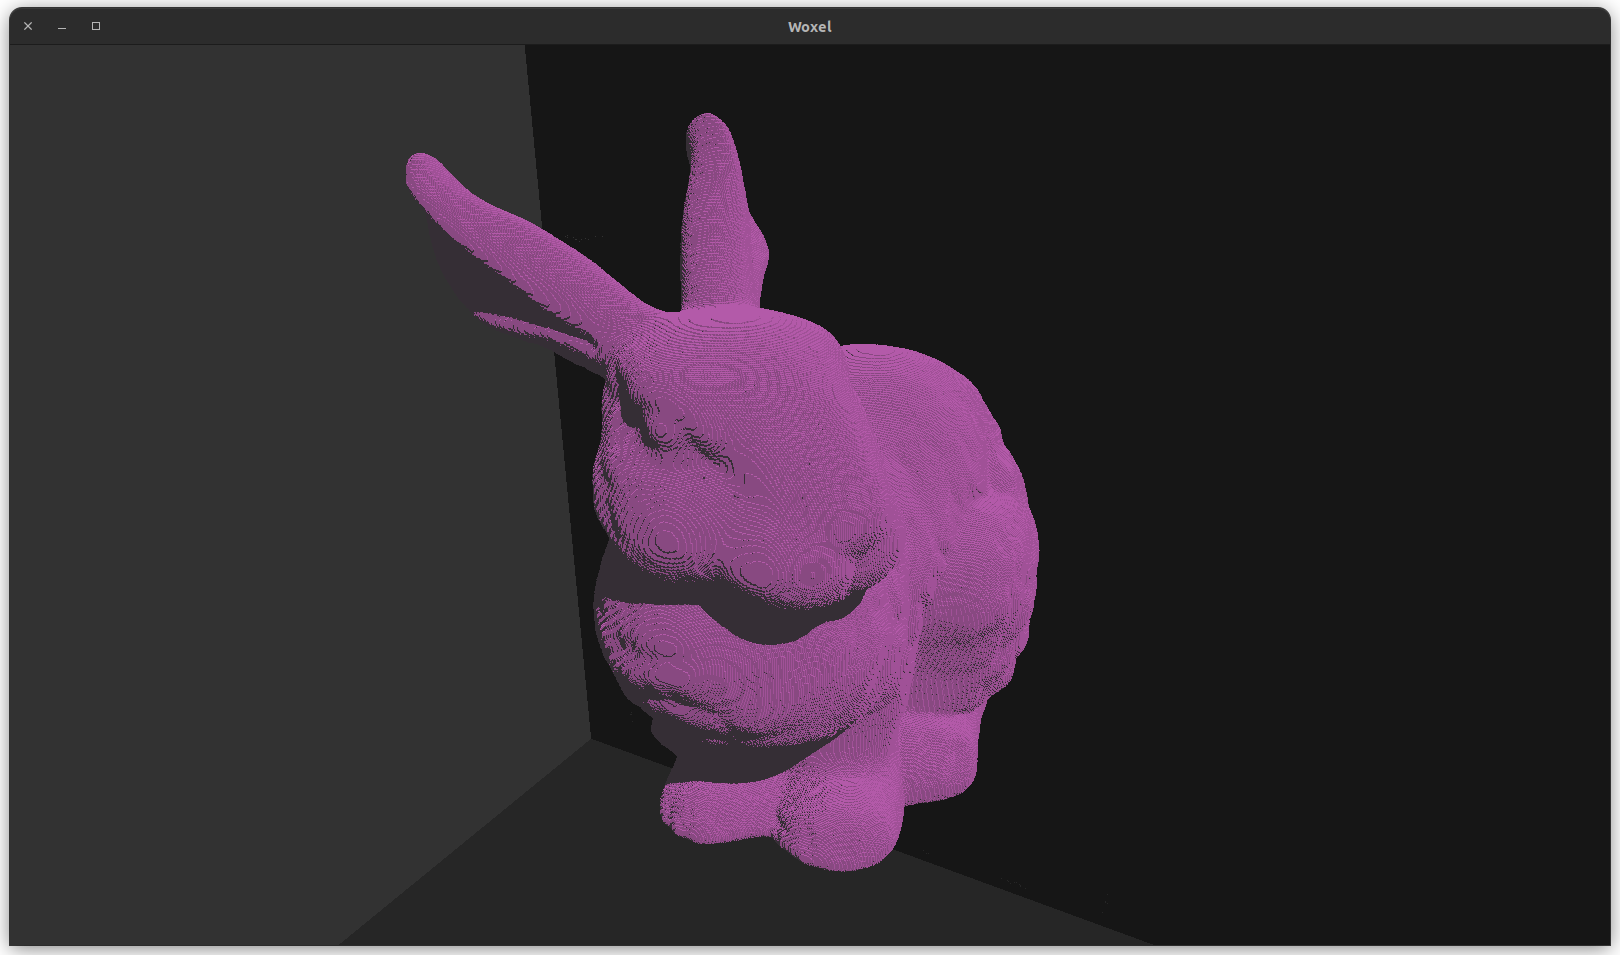
\includegraphics[width=0.8\textwidth]{bunny}
  \caption{Bunny with diffuse pink material, model voxel resolution: $628\times621\times489$}
\end{figure}

\section{Images}

This section shows some images captured in the rendering engine. All the models used are samples from the OpenVDB website\supercite{openvdb:models}. Each of the figures bellow showcase a different functionalities of the engine.

\begin{figure}[H]
  \centering
  \begin{subfigure}[b]{0.48\textwidth}
    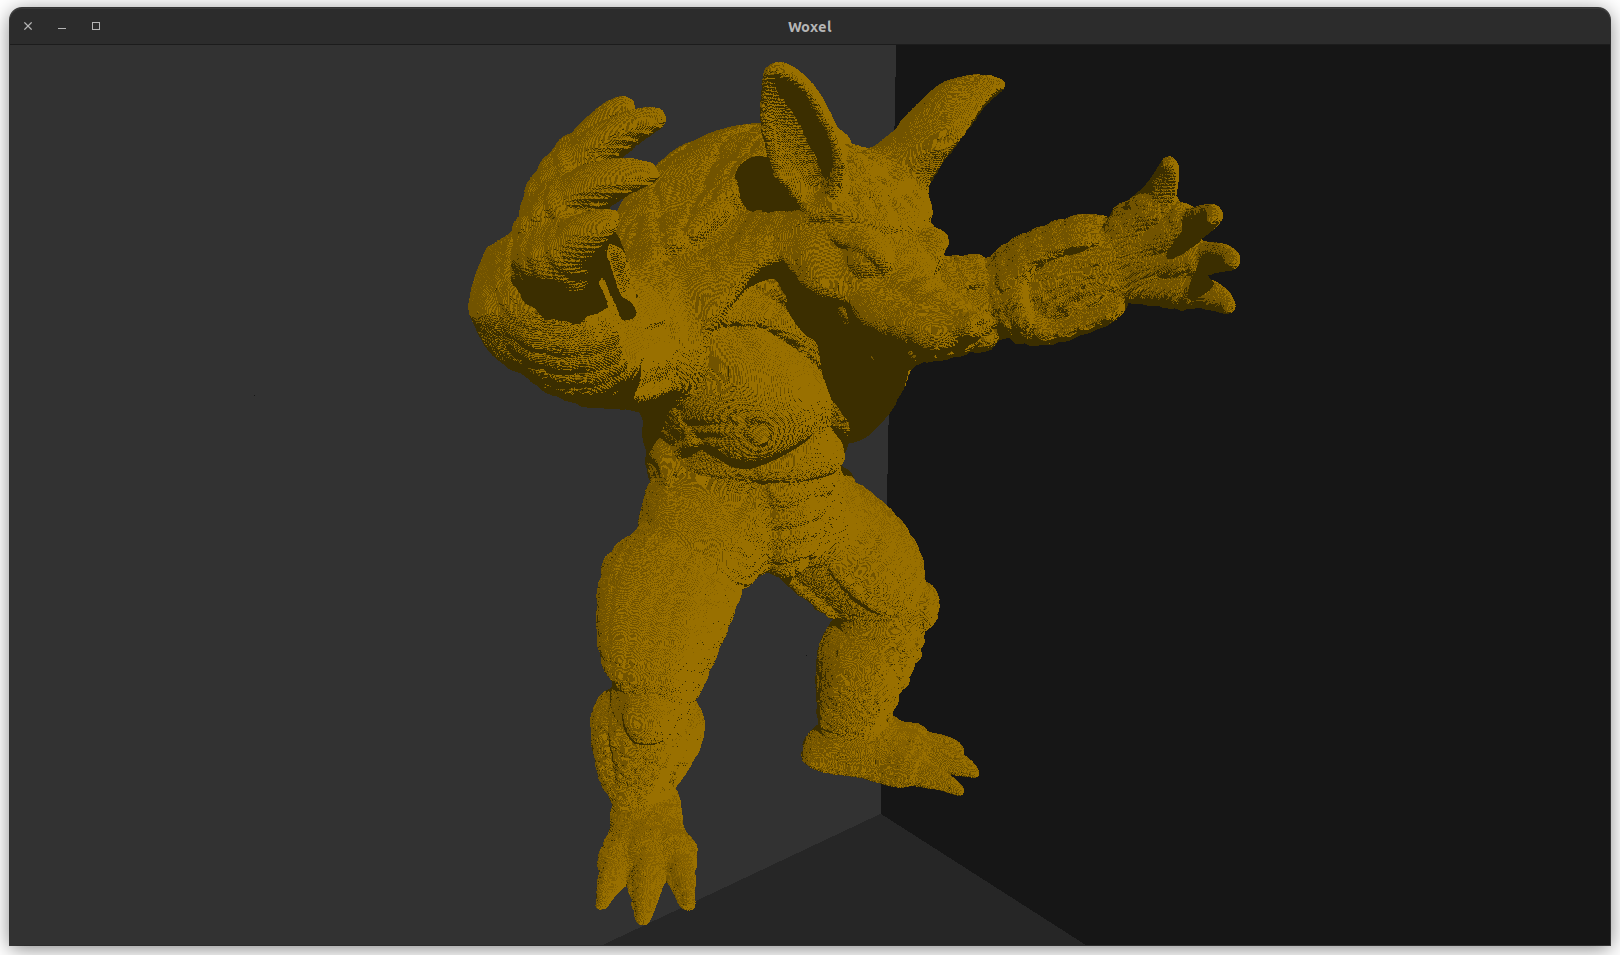
\includegraphics[width=\textwidth]{arm_1}
  \end{subfigure}
  \hfill
  \begin{subfigure}[b]{0.48\textwidth}
    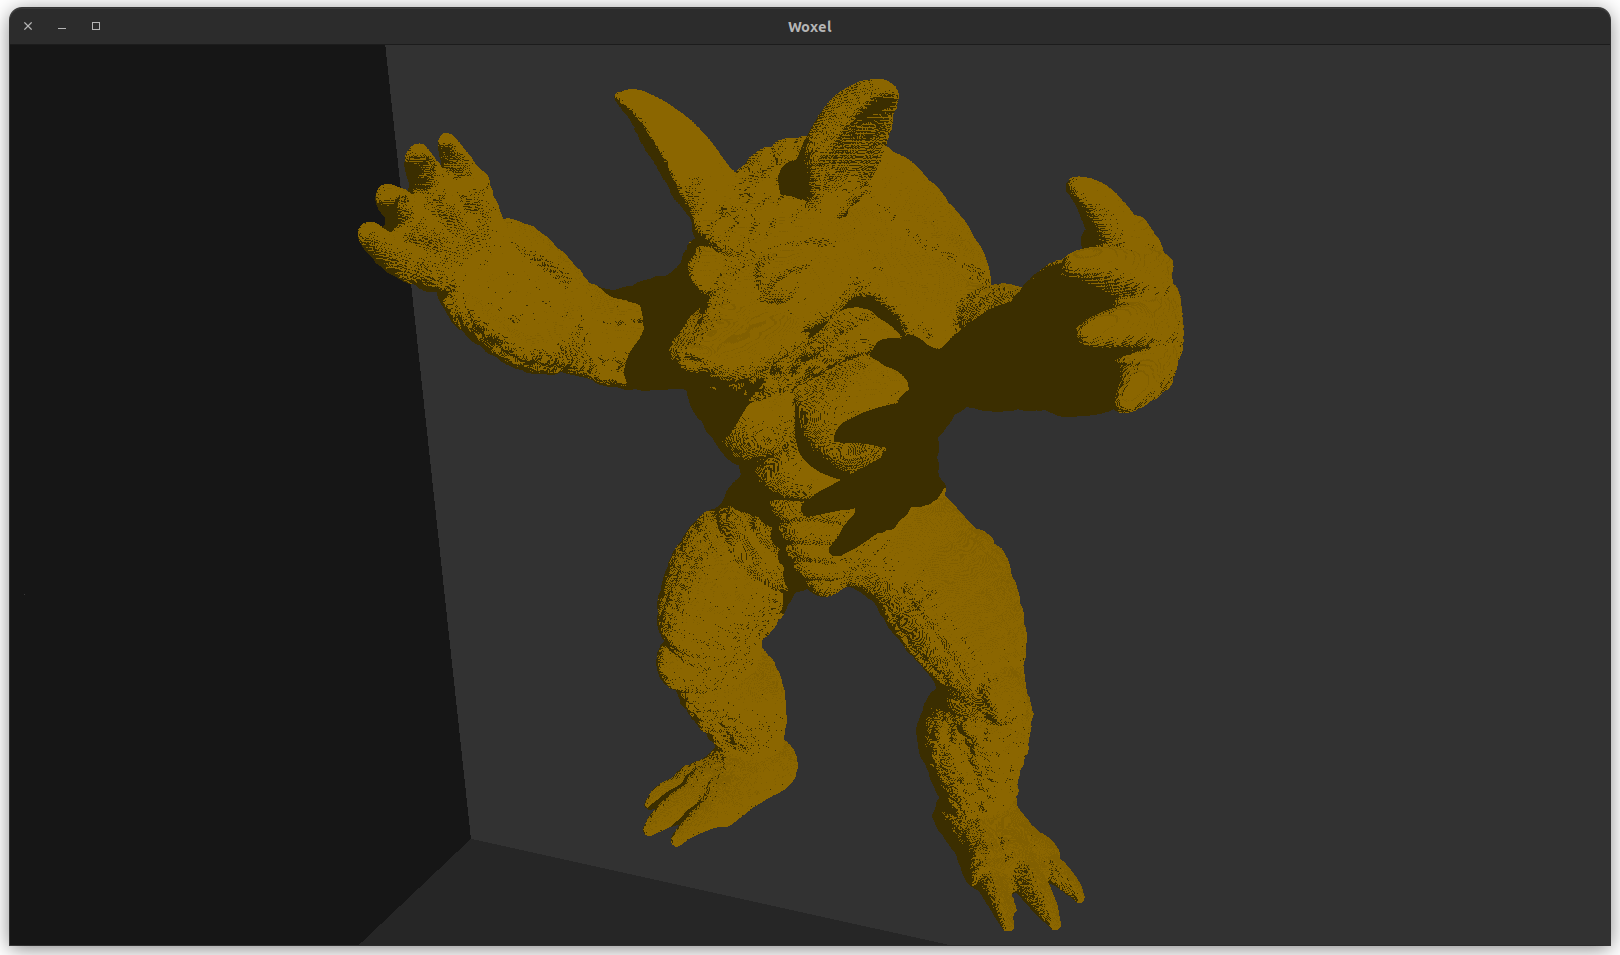
\includegraphics[width=\textwidth]{arm_2}
  \end{subfigure}
  \begin{subfigure}[b]{0.48\textwidth}
    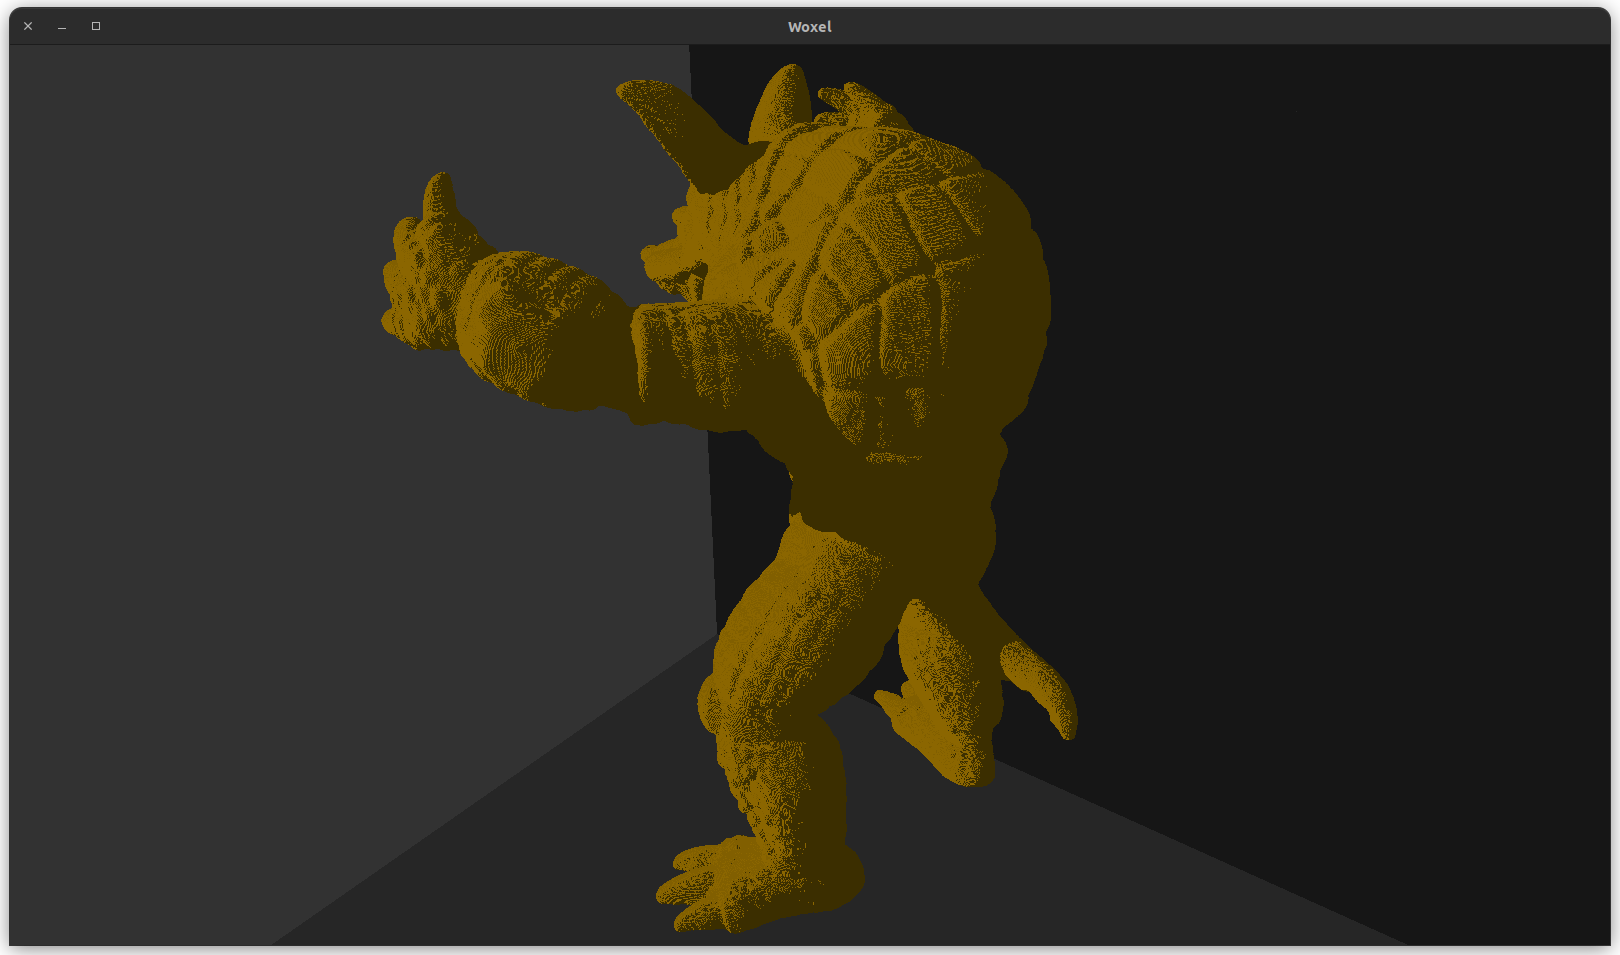
\includegraphics[width=\textwidth]{arm_3}
  \end{subfigure}
  \hfill
  \begin{subfigure}[b]{0.48\textwidth}
    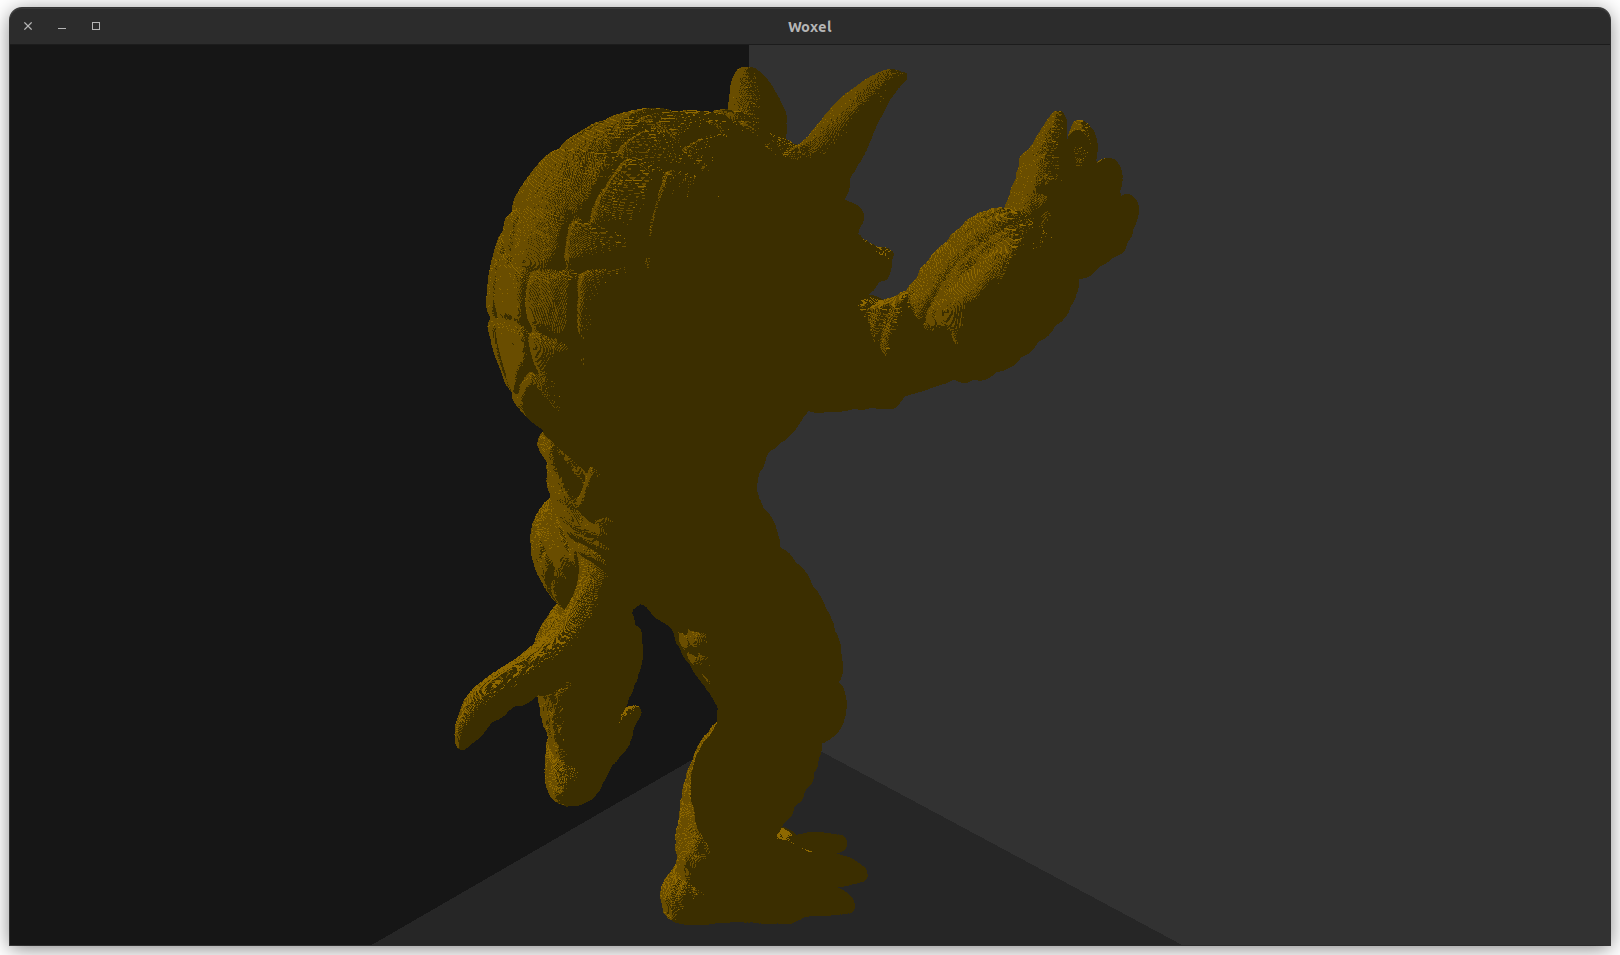
\includegraphics[width=\textwidth]{arm_4}
  \end{subfigure}
  \caption{\textbf{Multiple angles} of an armadilo model with a diffuse material. The voxel resolution of the model is $1276\times1518\times116$}
\end{figure}

\newacronym{iss}{ISS}{International Space Station}
\begin{figure}[H]
  \centering
  \begin{subfigure}[b]{0.48\textwidth}
    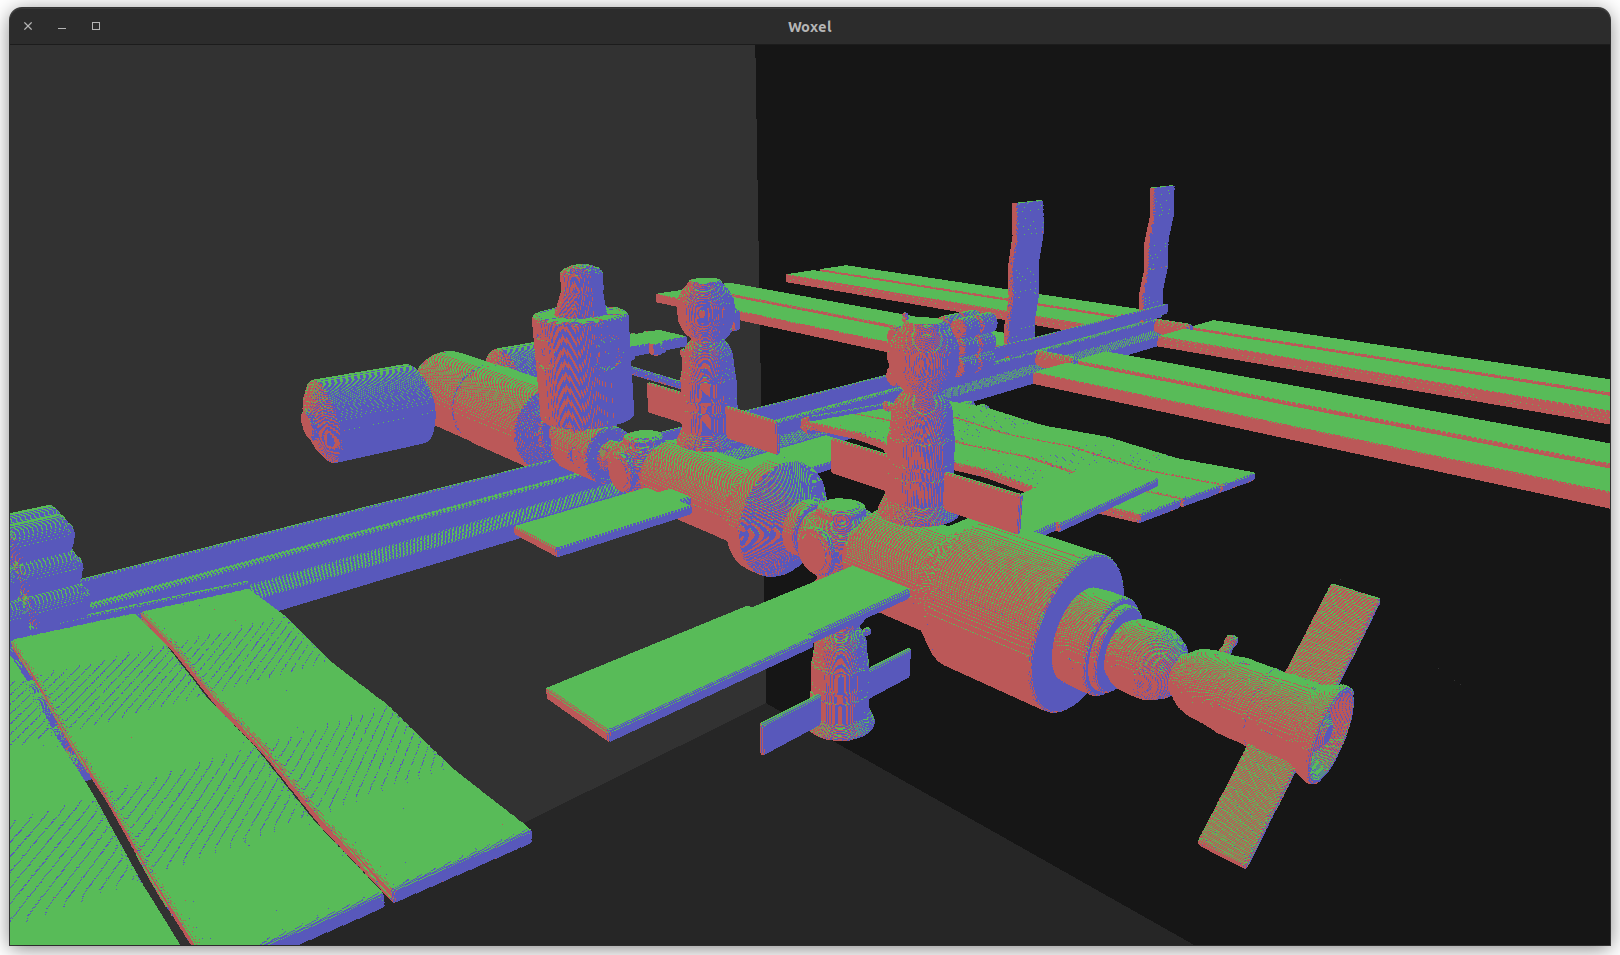
\includegraphics[width=\textwidth]{iss_rgb}
    \caption{RGB}
  \end{subfigure}
  \hfill
  \begin{subfigure}[b]{0.48\textwidth}
    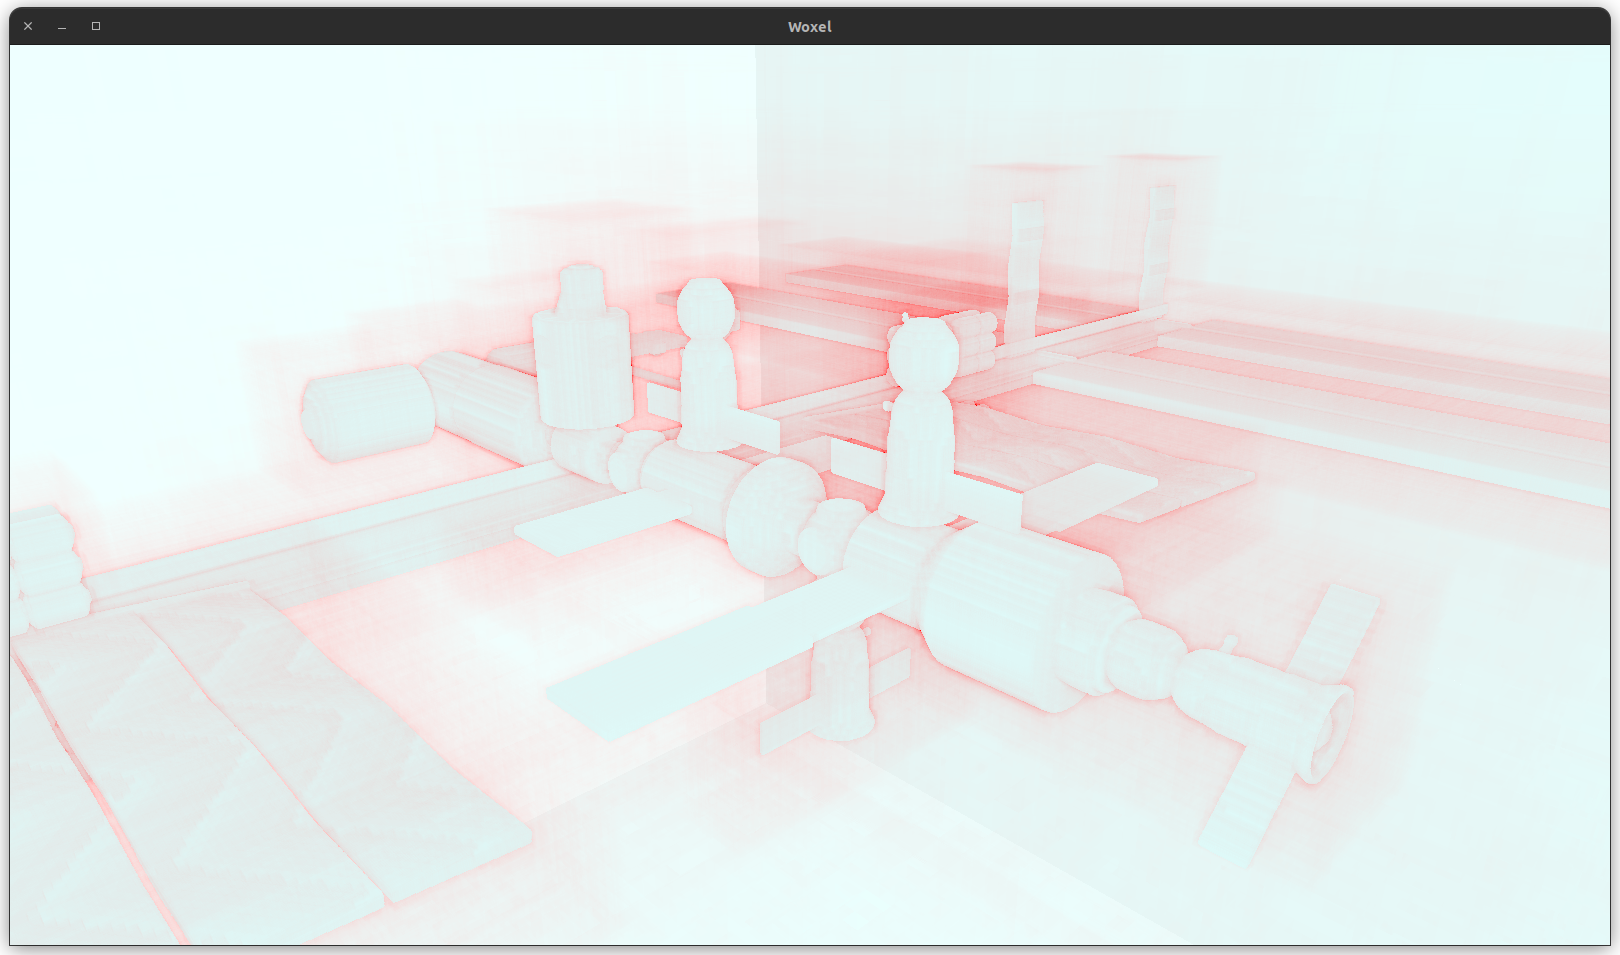
\includegraphics[width=\textwidth]{iss_ray}
    \caption{Ray}
  \end{subfigure}
  \begin{subfigure}[b]{0.48\textwidth}
    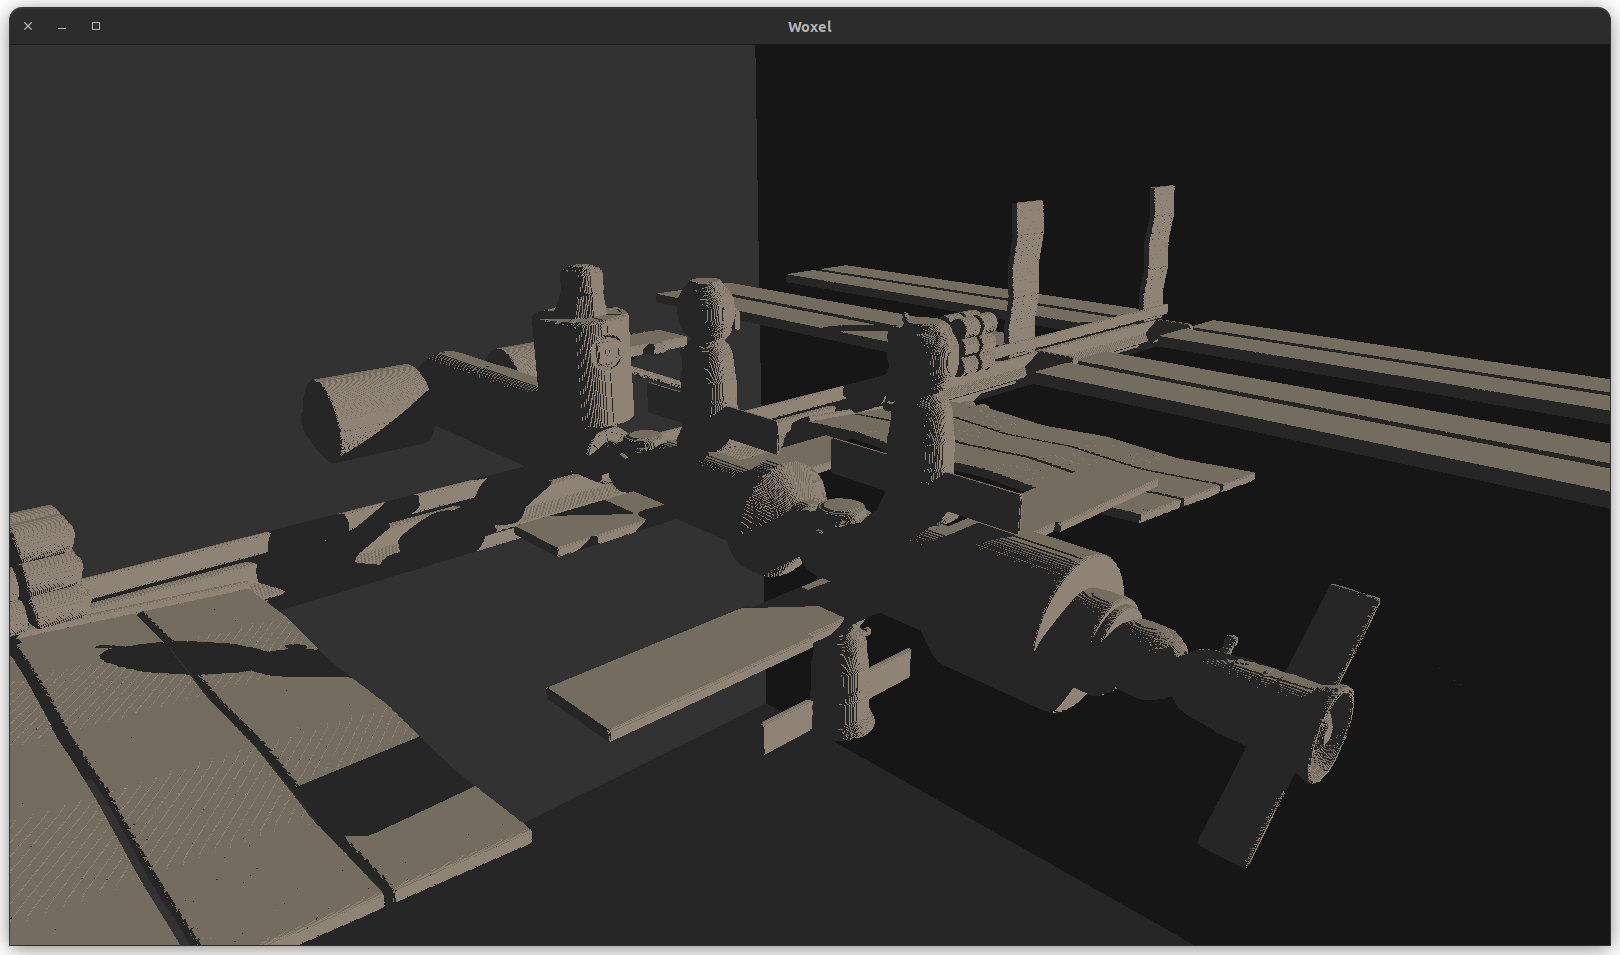
\includegraphics[width=\textwidth]{iss_diffuse}
    \caption{Diffuse}
  \end{subfigure}
  \hfill
  \begin{subfigure}[b]{0.48\textwidth}
    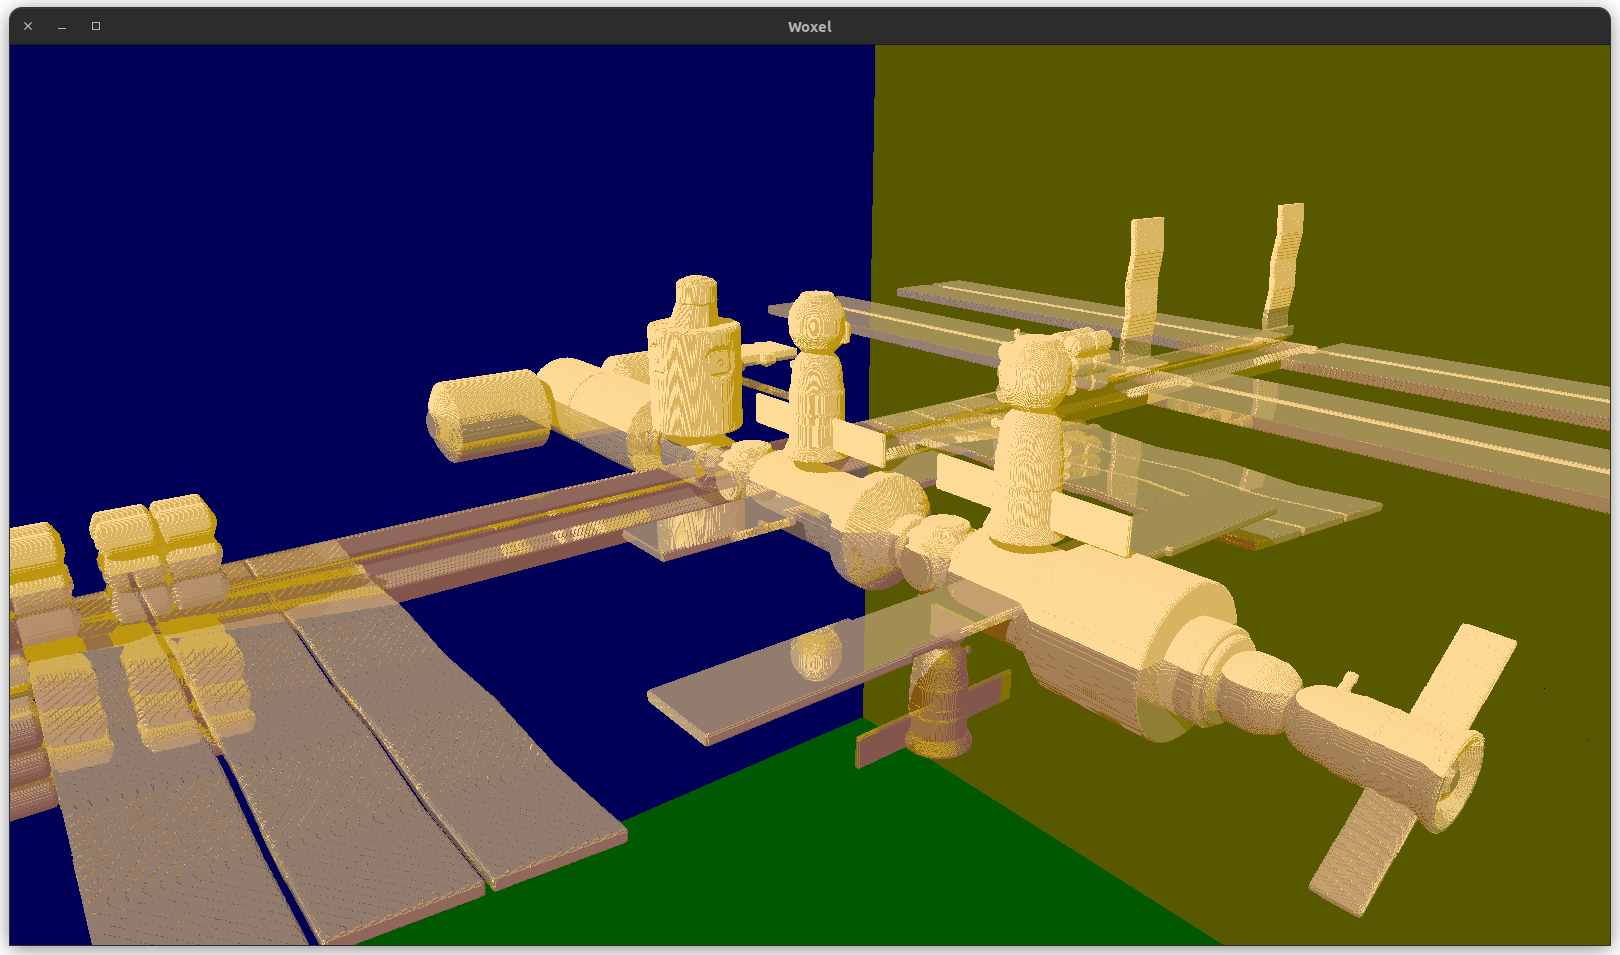
\includegraphics[width=\textwidth]{iss_gloss}
    \caption{Glossy}
  \end{subfigure}
  \caption{\textbf{Render modes} on a \acrshort{iss} model with voxel resolution $4561\times617\times2999$
    (a): RGB mode colors each face based on what axis it is parallel to.
    (b): Ray mode colors each pixel based on how many steps the ray took. The color is interpolated between light blue and red based on how many steps the ray took to go out of bounds or intersect a voxel. Maximum (red) is 200 steps.
    (c): Diffuse mode shows an object with diffuse material lit by sunlight.
    (d): Glossy mode shows a half glossy (bottom), half diffuse (top) model lit by sunlight. The out of bounds box is colored to discriminate which is face reflected on what surface. The reflection of the middle pod with a sphear on top can be seen in the solar panel in the middle. More reflections can be seen in the solar panels one the left and right.
  }
  \label{rendermods}
\end{figure}


\begin{figure}[H]
  \centering
  \begin{subfigure}[b]{0.48\textwidth}
    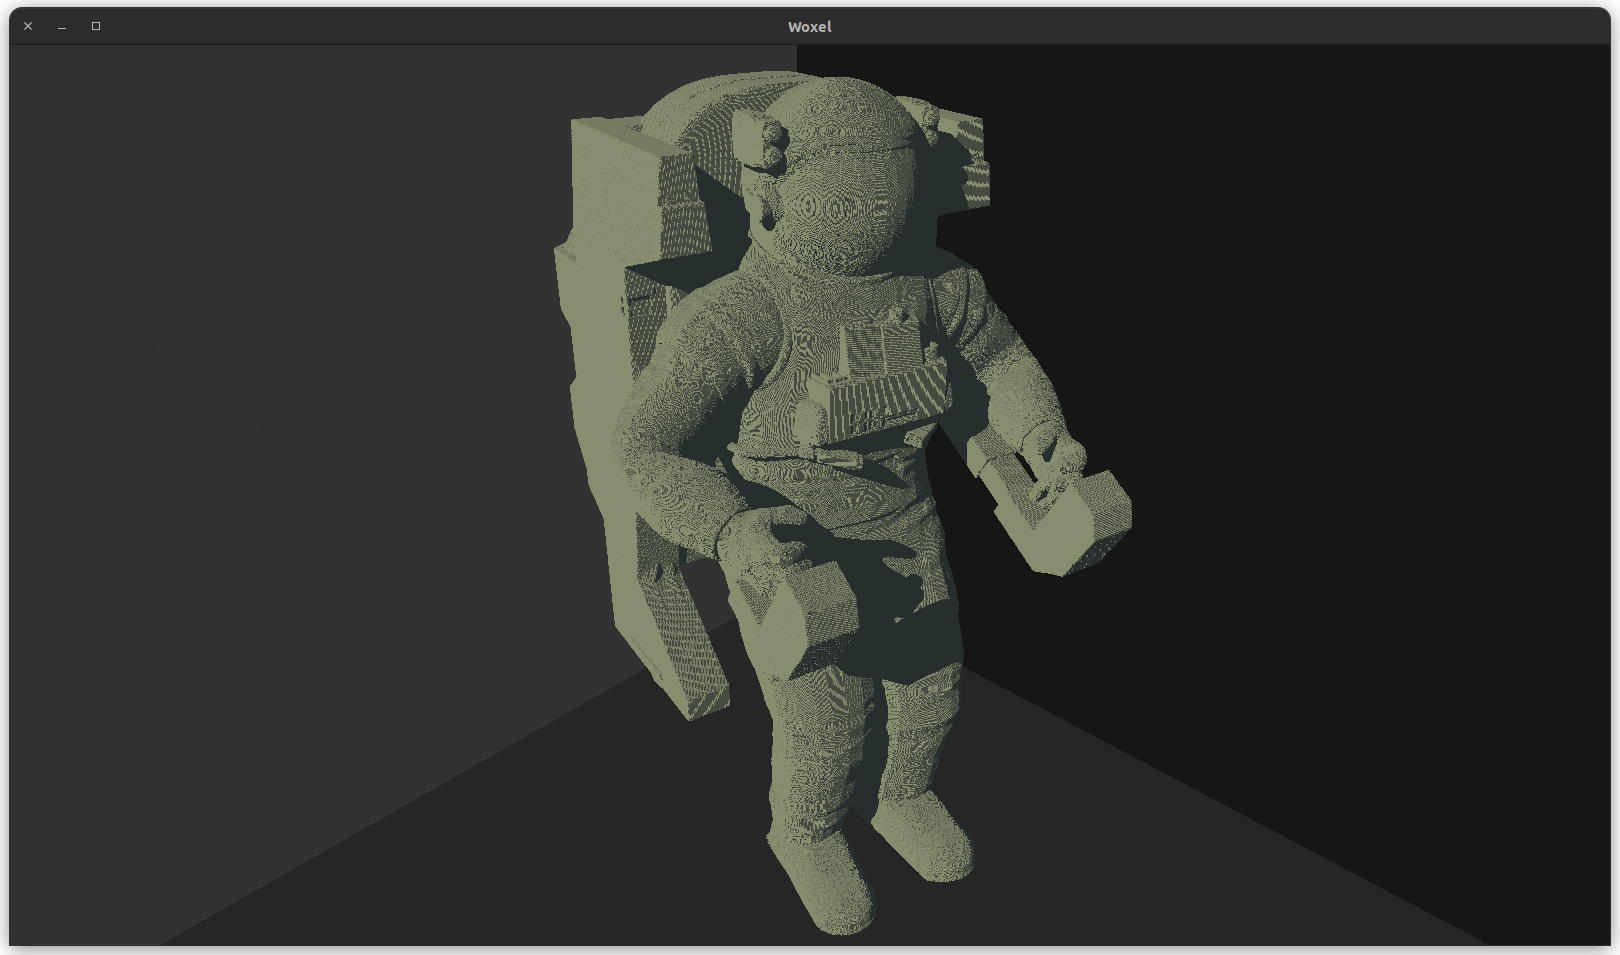
\includegraphics[width=\textwidth]{astro_1}
  \end{subfigure}
  \hfill
  \begin{subfigure}[b]{0.48\textwidth}
    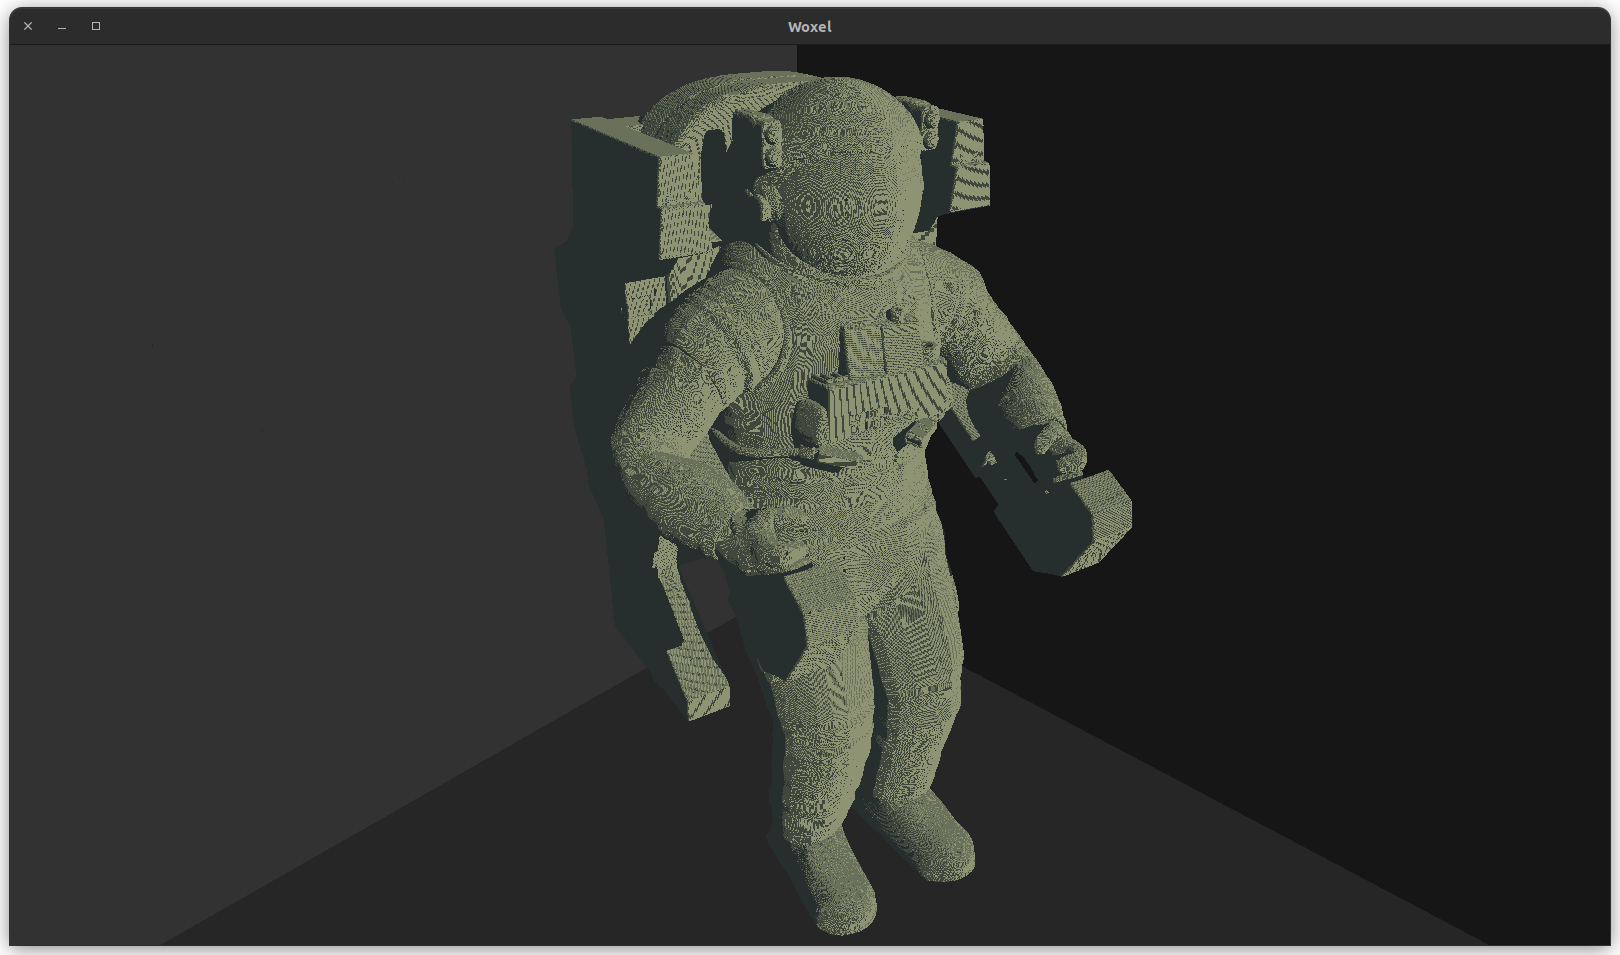
\includegraphics[width=\textwidth]{astro_2}
  \end{subfigure}
  \begin{subfigure}[b]{0.48\textwidth}
    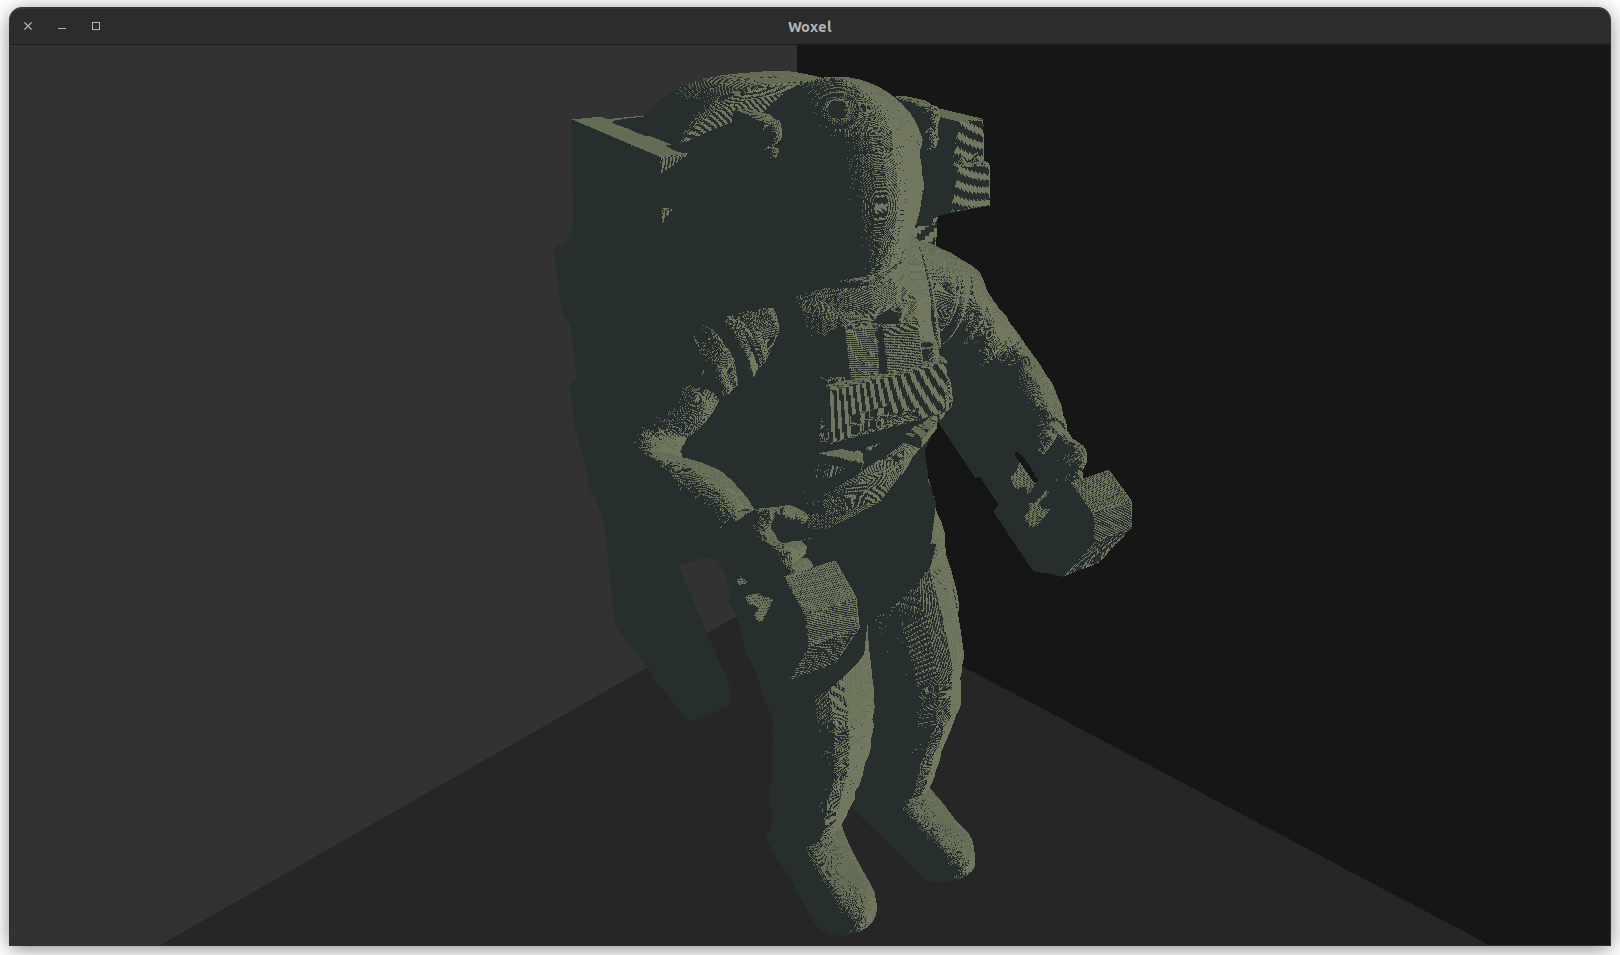
\includegraphics[width=\textwidth]{astro_3}
  \end{subfigure}
  \hfill
  \begin{subfigure}[b]{0.48\textwidth}
    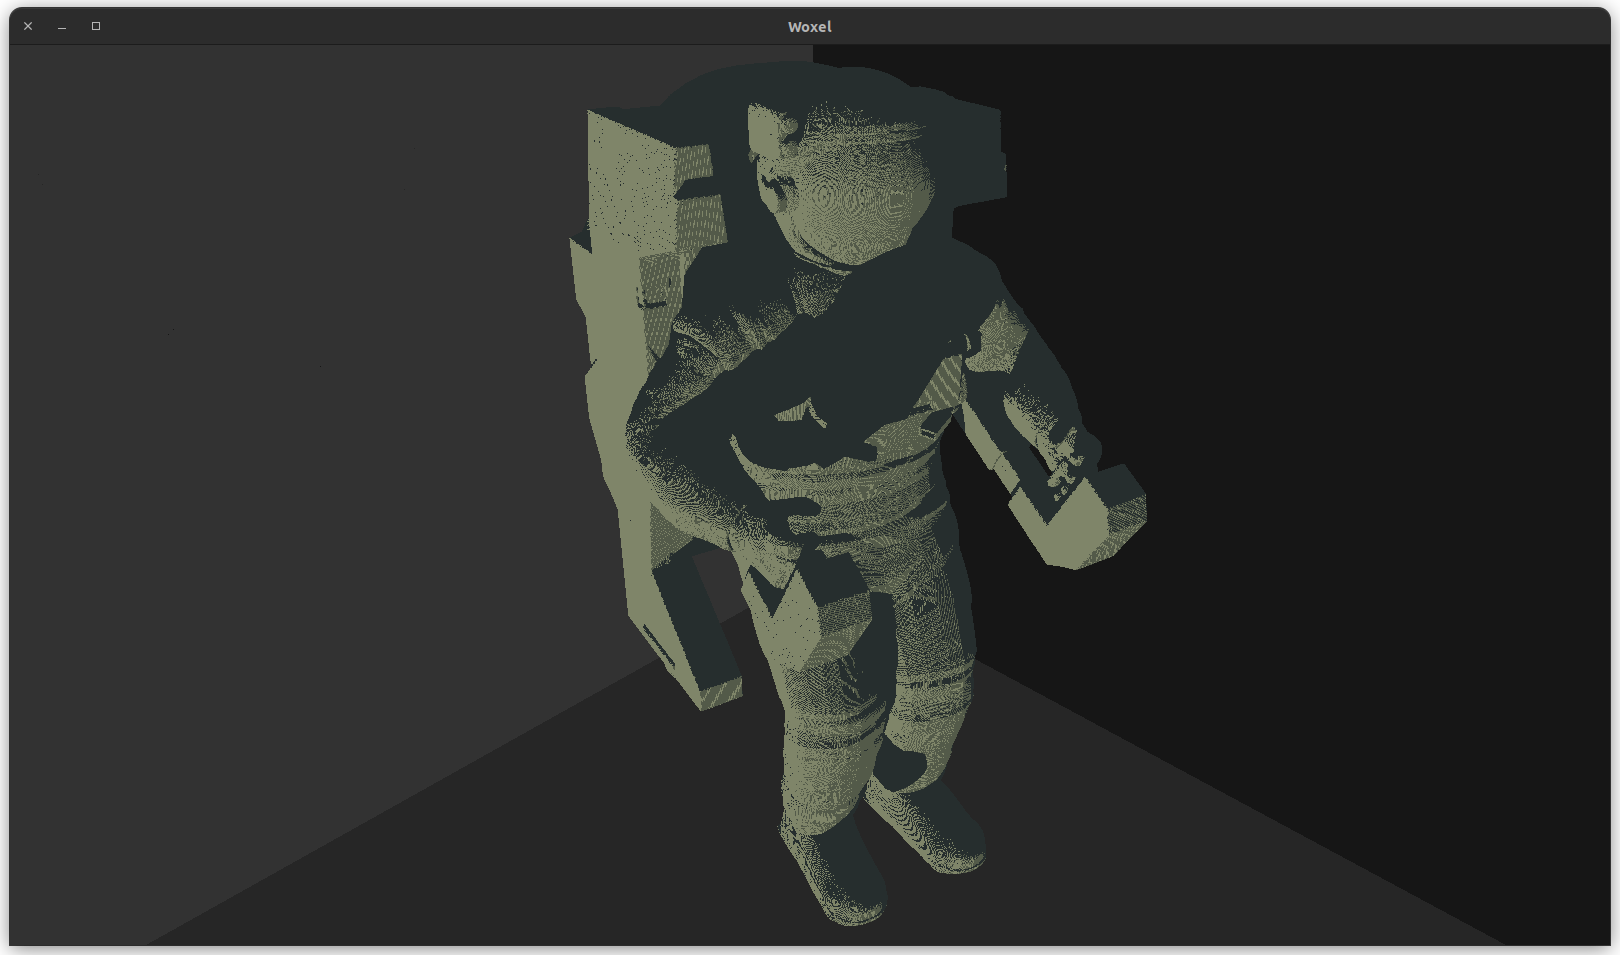
\includegraphics[width=\textwidth]{astro_4}
  \end{subfigure}
  \caption{\textbf{Dynamic Lighting} on an astronaut model. The sunlight is dynmaic, its direction, color and intensity can be changed through the developer GUI in real-time. The voxel resolution of the model is $1481\times2609\times1843$}
\end{figure}

\begin{figure}[H]
  \centering
  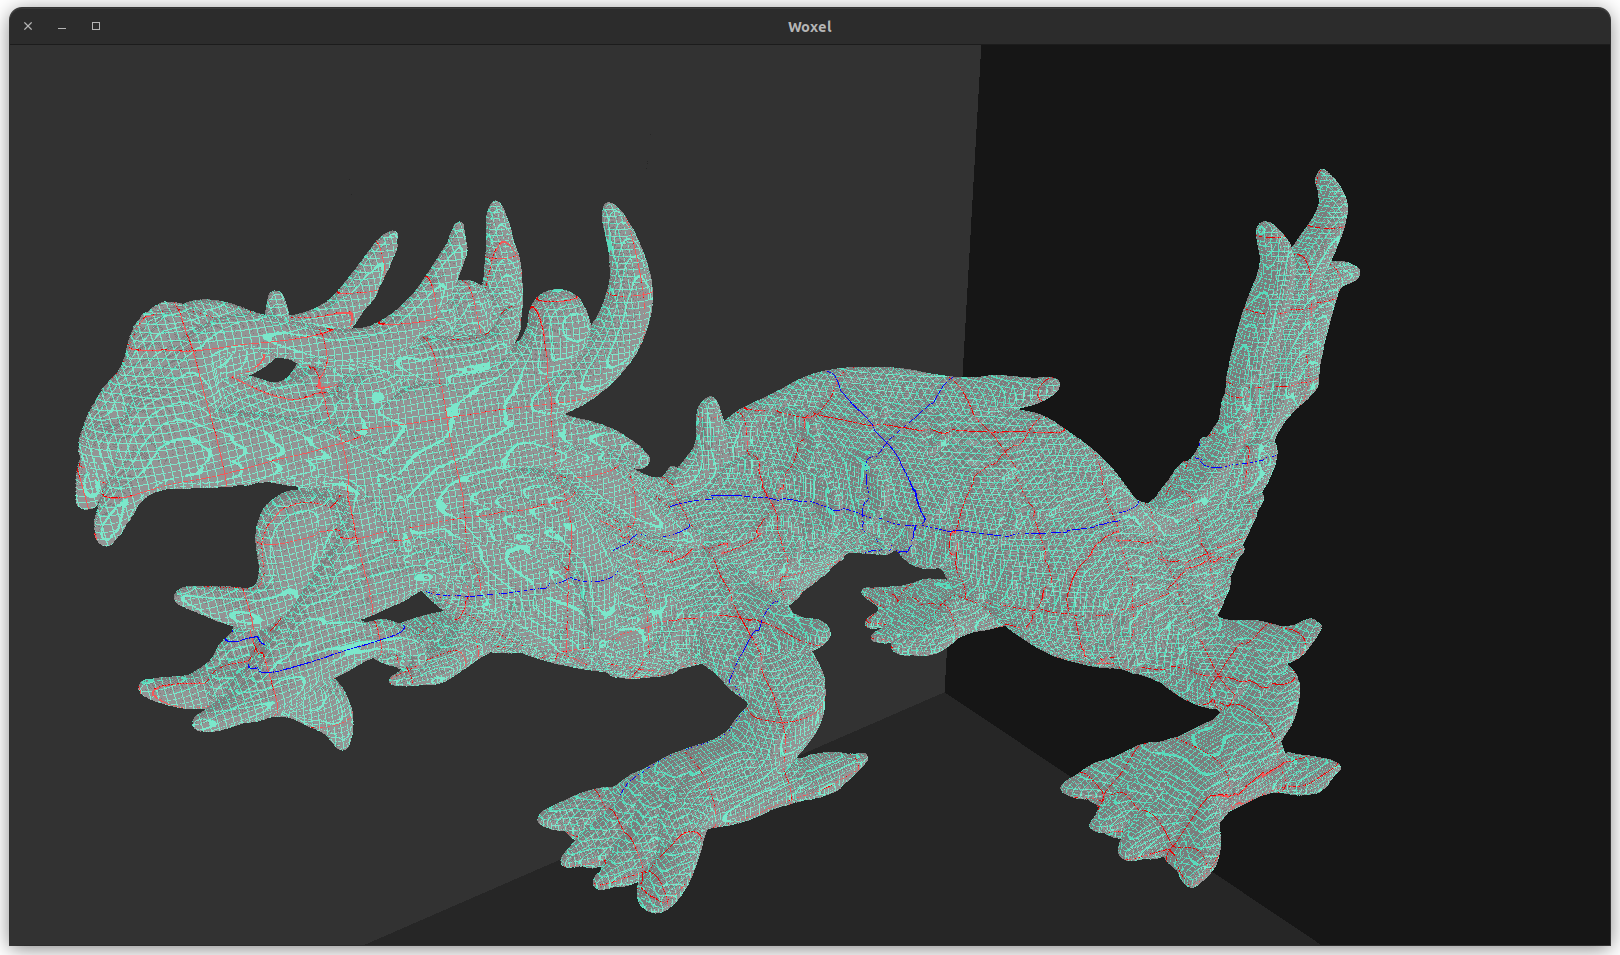
\includegraphics[width=0.8\textwidth]{dragon_3}
  \caption{\textbf{VDB highligthing}: Voxels at the boundries of VDB nodes are highlighted on a dragon model. The grid structure of the VDB can be seen at each level in the hierarchy. Node3, Node4 and Node5 boundries are shown in Cyan, Red and Blue respectively. The voxel resolution of the model is $2023\times911\times1347$}
\end{figure}

\begin{multicols}{2}[]
  \begin{figure}[H]
    \centering
    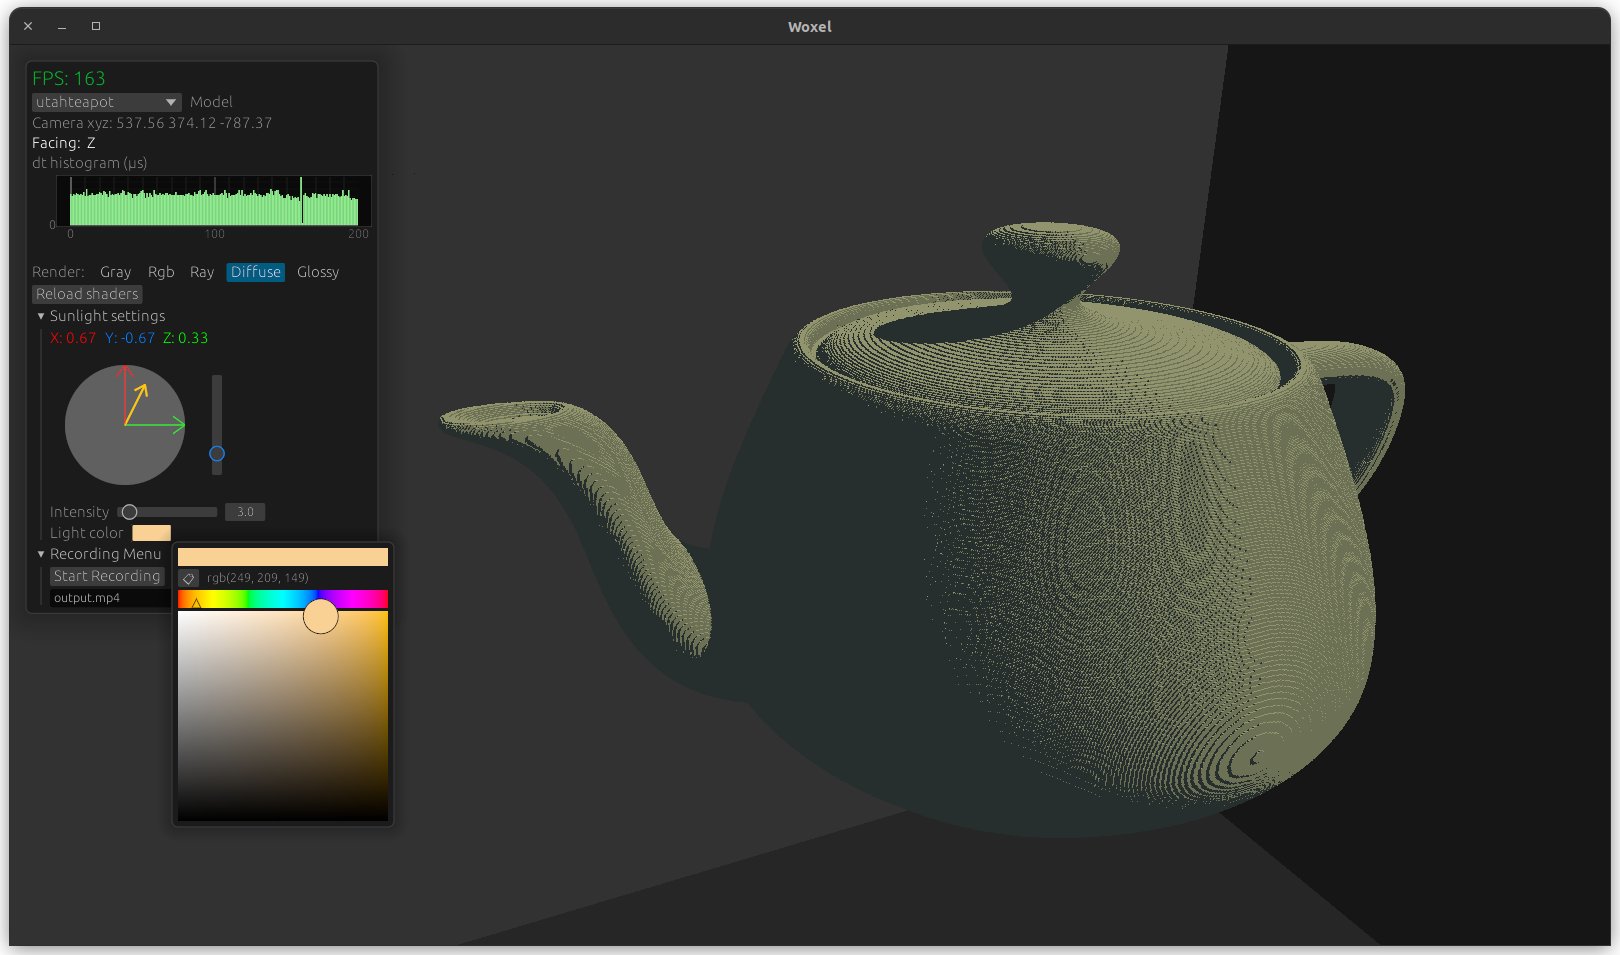
\includegraphics[width=0.96\linewidth]{gui_1}
    \caption{Developer GUI in engine}
  \end{figure}
  The developer GUI has the following uses:
  \begin{enumerate}[itemstep=0mm]
    \item Display current \acrshort{FPS} and histogram of milliseconds per frame.
    \item Changing the model in the viewport through a drop down menu that scans the assets folder for available models.
    \item Camera coordinates and facing direction
    \item Functionality to change between the render modes presented in \cref{rendermods}
    \item The option to reload the shaders while the engine is running.
    \item For the diffuse and glossy render modes there is a sunlight section available.
    \item The recording menu allows setting an output file and starting or ending the recording.
  \end{enumerate}
  \columnbreak
  \begin{figure}[H]
    \centering
    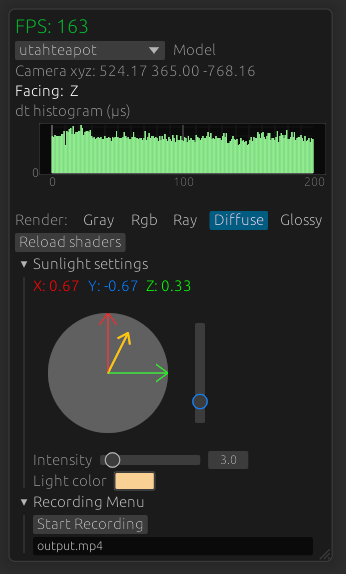
\includegraphics[width=1.0\linewidth]{gui_2}
    \caption{Developer GUI close-up}
    \label{gui}
  \end{figure}
\end{multicols}

\section{Experiments}
In this section the ray catsing algorithms are compared against each other on different models and render modes.

The specifications of the machine the experiments where ran on are presented in \cref{specs}.
\begin{table}[h]
  \centering
\begin{tabular}{|c||c|}
  \hline
  \multicolumn{2}{|c|}{Experiment machine specifications} \\
  \hline
  OS & Ubuntu 22.04.3 LTS x86\_64\\
  \hline
  CPU & AMD Ryzen 7 5800H with Radeon\\
  \hline
  GPU &  NVIDIA GeForce RTX 3070 Mobile\\
  \hline
  RAM & 8192MiB \\
  \hline
  FMA & Enabled \\
  \hline
\end{tabular}
  \caption{Experiment machine specifications}
  \label{specs}
\end{table}

\subsection{Comparing DDA, HDDA and HDDA+SDF}

The average millseconds per frame are compared for the DDA, HDDA and HDDA+SDF algorithms on the teapot model (voxel resolution of $981\times462\times617$), on the ray render mode, at 3 distinct distances from the model, one further a way, ore closer and one near the model. Checking at three separate distances is important because the performance of the hierarchical algorithms depends on the topology that the camer rays are going through. When the target object is fur away most camera rays are able to traverse the VDB at hiegher levels in tree since there is no detail around. Conversly, when the camera is closer to the object the rays must treverse more complex topolgy at lower levels in the tree, and therfore the aglorithm can be slower.

\begin{table}[h]
  \centering
  \begin{tabular}{|c||c|c|c|}
    \hline
    & 2000m & 1000m & 500m \\
    \hline
    DDA & 100.3ms* & 100.1ms* & 50.4ms \\
    \hline
    HDDA & 9.4ms & 12.5ms & 14.4ms \\
    \hline
    HDDA+SDF & 6ms** & 6.4ms & 7.6ms\\
    \hline
  \end{tabular}
  \caption{Milliseconds per frame of rendering the teapot model using DDA, HDDA, HDDA+SDF at far, medium, and close distance. A voxel is considered $1\rm{m}\times1\rm{m}\times1\rm{m}$. The average ms per frame is taken from a 1000 frame interval.\\
    *: Model doesn't show up in viewport because the algorithm exceeds the maximum step size of 1000. This time can be treated as the worst-case, casting bouncing the maximum number of times for each pixel.\\
    **: Frame rate cap is hit at 165 FPS, this is as good as the ray casting can get on this machine}
\end{table}

\begin{figure}[H]
  \centering
  \begin{subfigure}[b]{0.48\textwidth}
    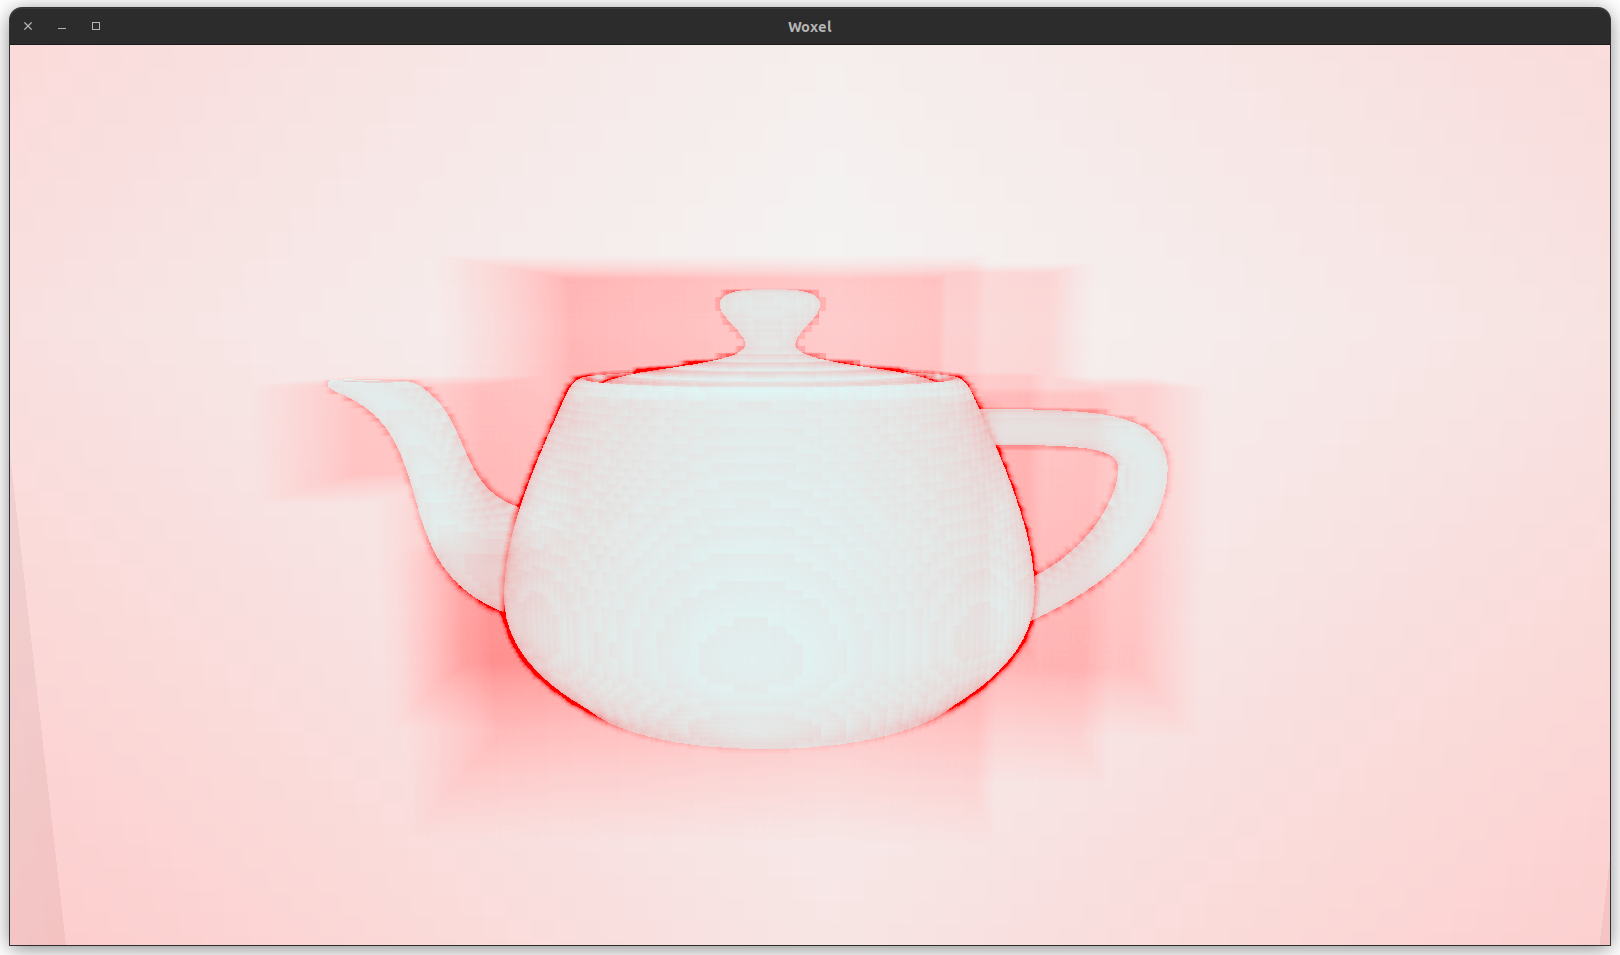
\includegraphics[width=\textwidth]{teapot_2}
    \caption{}
  \end{subfigure}
  \hfill
  \begin{subfigure}[b]{0.48\textwidth}
    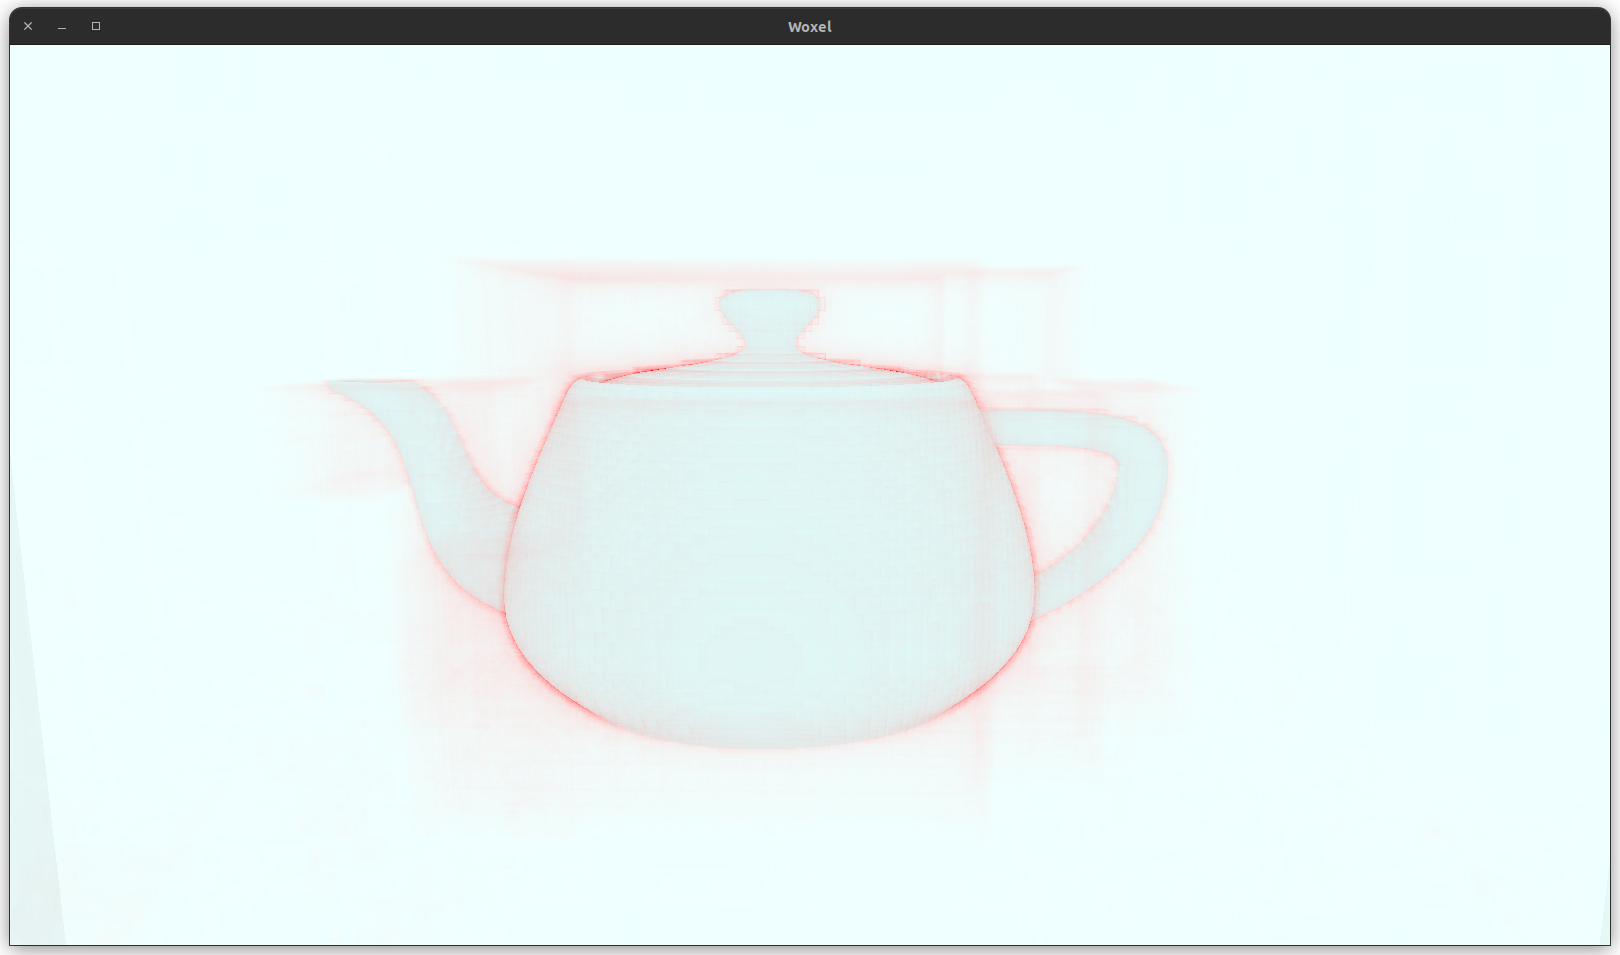
\includegraphics[width=\textwidth]{teapot_1}
    \caption{}
  \end{subfigure}
  \caption{Render in ray mode using (a) HDDA and (b) HDDA+SDF of the teapot model from 1000m distance. The model resolution is: $981\times462\times617$. As in \cref{rendermods}(b) the color of pixels is determined based on the steps the ray took to intersect the model. The maximum is 200 steps corresponding to bright red.}
  \label{teacomp}
\end{figure}

The DDA version cannot handle a mesh of this resolution, since rays are marched one voxel at a time. At 2000 voxels away, no ray can get to the object before it exceeds the maximum step rate of 1000. At 500 voxels away the DDA manages to render part of the teapot at 50 milliseconds per frame ($20$ FPS) which is not enough for modern engines.
Both the HDDA and HDDA+SDF perform very well on this model. The HDDA algorihtm has a minimum FPS at the 500m point of 70 FPS. The HDDA+SDF manages to hit the frame rate cap of the GPU at 165 FPS at the 2000m point and doesn't drop bellow 120 FPS at the close point. Adding the SDF to the HDDA algorithm yeilds a performance boost of $36\%$ at 2000m, $49\%$ at 1000m and $47\%$ at 500m.

It is visible in \cref{teacomp} that the most of the improvment that the SDF offers is actually for pixels whos corresponding camera rays don't actually intersect voxels. This is because these voxels are intersected relatively quickly in the classic HDDA. The slowest raycasting operations are those that pass voxels very close by and go then off  into the background, as showed in \cref{steps}. This is precisely where the SDF is most useful, since it can get the ray to get out of those high detail areas faster. Moreover, when the ray travelling in low detail space there is also an improvment because the further the ray gets from the object the further it will step. This allows rays to get out of bounds as much faster.

\begin{figure}[H]
  \centering
  \includesvg[width=0.5\textwidth]{steps.svg}
  \caption{ray that intersects voxel vs. ray that ``near-misses'' it. The first has 2 axis crossings, the latter has 9.}
  \label{steps}
\end{figure}

The same experiment setup is repeated for the ISS model because it has a lot of gaps and tight spaces in it's geometry, this time only HDDA and HDDA+SDF is considered since the DDA could not handle the teapot model, which is much smaller than the ISS. Another change is the camera positions used are no longer based on the distance to the object, and are instead positioned such that increasing levels of detail and overlapping geometry is in view.

\begin{table}[h]
  \centering
  \begin{tabular}{|c||c|c|c|}
    \hline
    & pos. 1 & pos. 2 & pos. 3 \\
    \hline
    HDDA & 9.1ms & 10.6ms & 15.3ms \\
    \hline
    HDDA+SDF & 6ms** & 7.2ms & 8.3ms\\
    \hline
    improvement & 36\% & 32\% & 46\%\\
    \hline
  \end{tabular}
  \caption{Milliseconds per frame of rendering the \acrshort{iss} model using HDDA, HDDA+SDF at 3 positions in space slected to be increasingly detailed. The average ms per frame is taken from a 1000 frame interval. The improvment from HDDA to HDDA+SDF is also recorder. \\
    **: Frame rate cap is hit at 165 FPS, this is as good as the ray casting can get on this machine}
\end{table}

\begin{figure}[H]
  \centering
  \begin{subfigure}[b]{0.48\textwidth}
    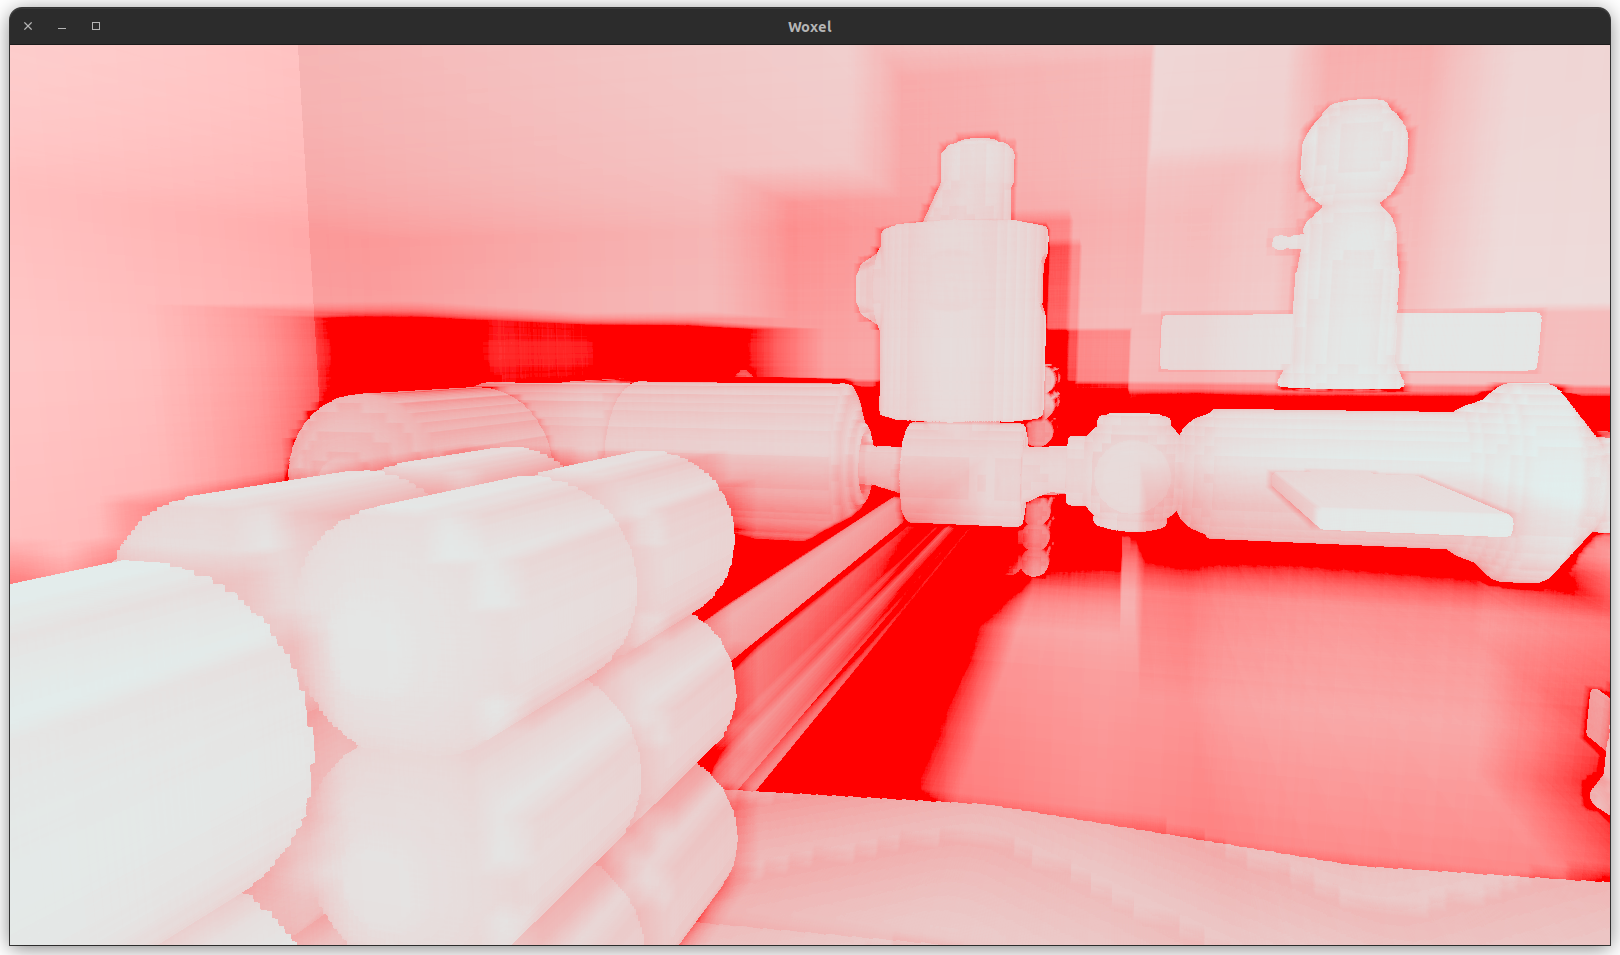
\includegraphics[width=\textwidth]{iss_hdda}
    \caption{}
  \end{subfigure}
  \hfill
  \begin{subfigure}[b]{0.48\textwidth}
    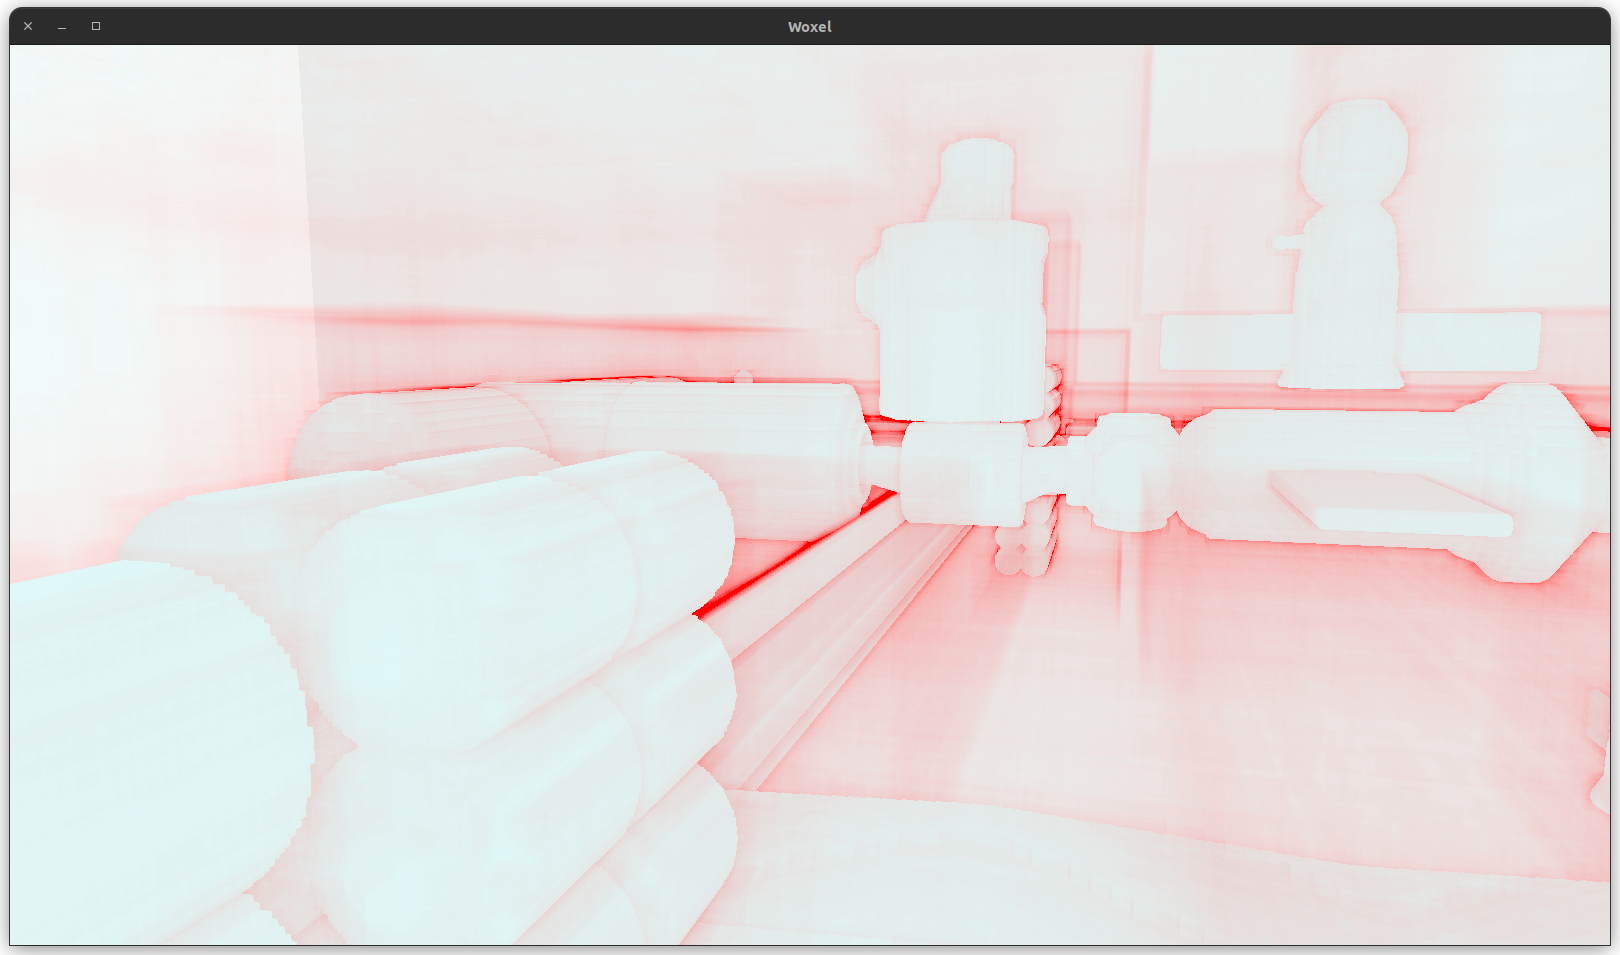
\includegraphics[width=\textwidth]{iss_sdf}
    \caption{}
  \end{subfigure}
  \caption{Render in ray mode using (a) HDDA and (b) HDDA+SDF of the ISS model at position 3. The model resolution is: $4561\times617\times2999$. The color of pixels is determined analogus to \cref{teacomp}. The efficiency of the SDF method in high detail areas can be cleary seen by comparing the two images: red patches in the middle of the image get much lighter and bright red areas exist only very close to the model surface.}
\end{figure}

These two experiments prove the efficiency of the HDDA+SDF method, it gives more then 30 \% speedup over HDDA in all cases, and is able to hit the frame rate cap of 165 FPS in for most conditions. The high resolution of the test scenese used also proves HDDA+SDF is a robust ray-marching algorithm which is able to handle complex scenes with good performance.

\subsection{Performance of HDDA+SDF in ray-tracing}

To test the performance of HDDA+SDF when doing ray-tracing the avergae milliseconds per frame will be recorded

\section{Future work}

\section{Limitations}

\section{Final remarks}
